\begin{recipe}
[ %
        preparationtime = {\SI{1}{\hour}},
        portion = {\portion{Idk, how much do you like potatoes?}},
        source = {HeNine}
    ]{Pra\v{z}en krompir}

    \pretitle{{\color{gray}\Large Saut\'eed Potatoes}\vspace{-1.5ex}}

    \begin{figure}[p]
	        \centering
	        \makebox[\textwidth][c]{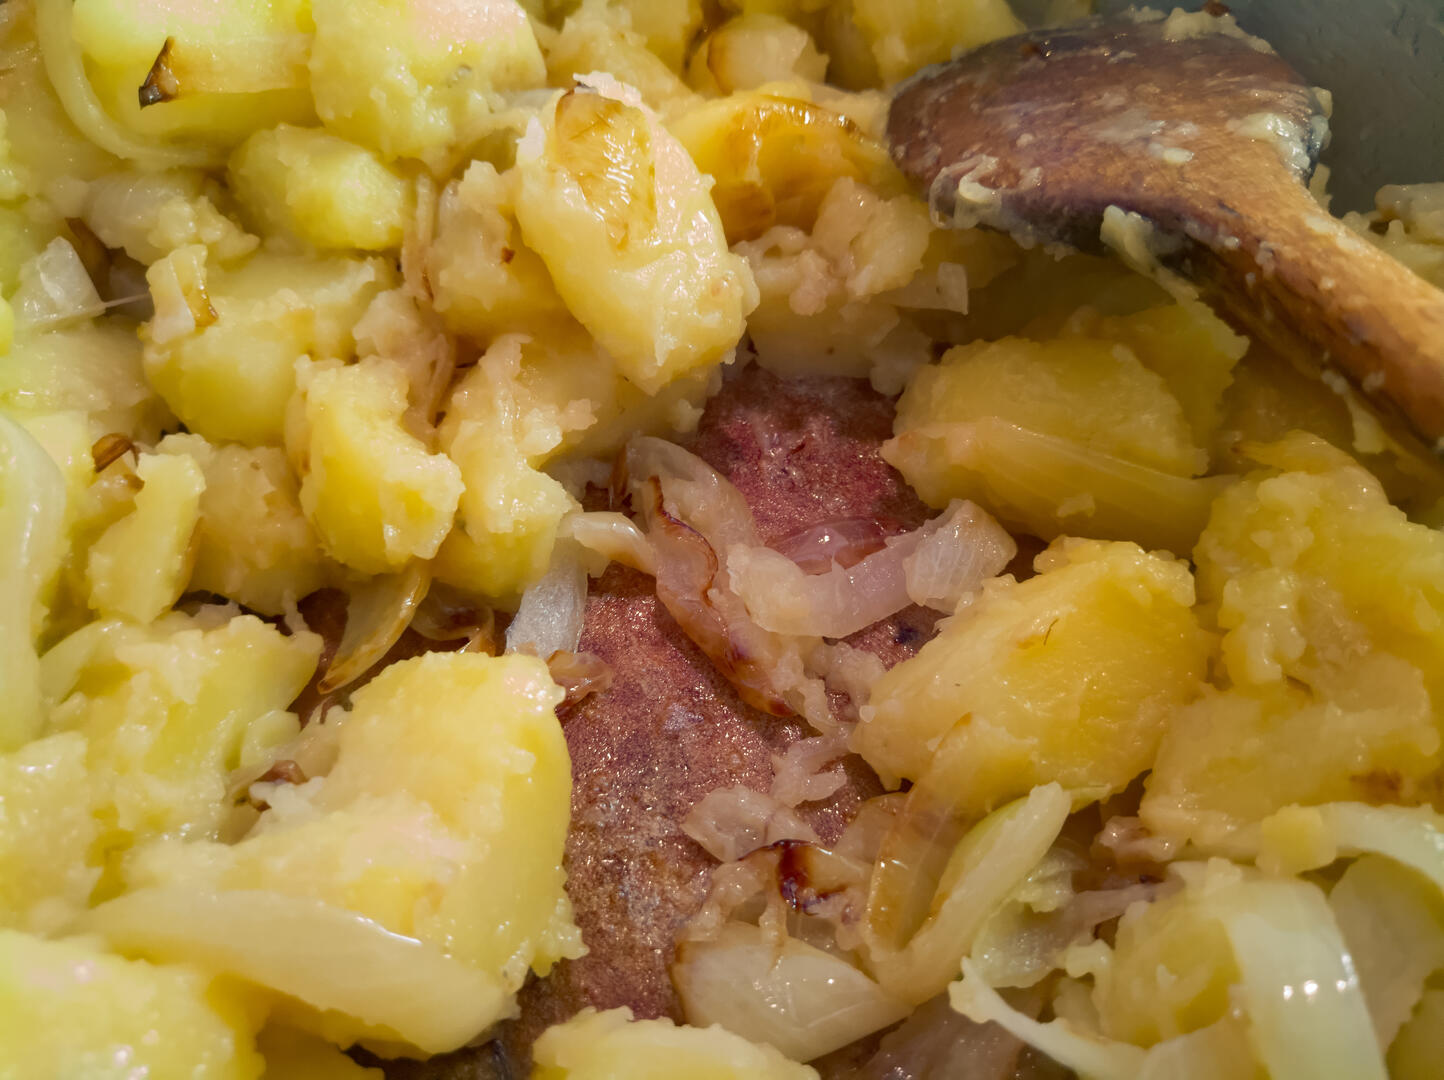
\includegraphics[height=\textheight]{prazen_krompir/IMG_20200409_114616.jpg}}
	    \end{figure}

    \introduction{
        This is a side dish that goes well with a nice roast or a \href{https://en.wikipedia.org/wiki/Carniolan_sausage}{Carniolan sausage}. Or eat it on its own, I’m not your mom.

        \textbf{\large Potatoes}

        Get the butteriest yellow potatoes you can find. Other potatoes may work, buy you’ll get pretty poor results with the starchier varieties.

        \textbf{\large Onion}

        Yellow or white works fine, red will completely ruin the color.
    }

    \ingredients[3]{
        2--3 & Medium potatoes \\
        1 & Medium to large onion \\
        & Salt and pepper
    }

    \preparation{
        \step Put whole, unpeeled, potatoes in water and bring to a boil. Boil until soft (test with fork or knife, knork is fine, spork is not; should take about 35 min.)

        (You can cook the potatoes well in advance and letting them cool makes them easier to peel.)

        \step Peel the potatoes. Cut them into mouthful-sized chunks. Slice the onion into rings or semi-circles.

        \step In a pan, fry the onion on high in a bit of oil until it starts to brown. Keep lightly stirring it so it browns, but doesn't burn, until most of it has at least some browning.

        \step Add the potatoes and salt, and lower the heat. Here is the tricky part: start stirring and scraping the potatoes off the bottom of your pan. You will not be able to get it ALL off and you should start to build a nice brown crust of potato on the bottom of your pan. THIS IS GOOD\footnote{Just make sure it doesn’t burn. It’s a delicate balance and I would recommend starting on low heat and raising it until it just starts to brown.}.

        While you do this, your potatoes will probably start to disintegrate into a chunky mash potato consistency. Keep stirring and building the crust until it’s nice and thick and feels like you will DEFINITELY not be able to scrape that off.

        \step Remove from heat, add the pepper\footnote{Pepper, pepper.} and give it one last stir. Cover with a lid and wait.

        \vspace{15em}

        \step The moisture will redistribute and soften your delicious potato crust. You should now be able to peel it off and mix it into the rest of potato-oniony goodness. If it doesn’t come off: cover and wait a bit longer.

        \step Serve.
    }

\end{recipe}